\section{Results}
\label{sec:results}

\subsection{Aging of a Fixed Phase and Effective Rates}
\label{sec:res_aging}
In this scenario the RIS carries most of the signal. With the direct links blocked, the median per-user SNR (channel gain over all BS antennas times $P/\sigma^2$) is 20.0~dB for the direct link alone and 31.1~dB for the RIS path with the SU-average phase. Without the RIS, the minimum user rate is 1.744~b/s/Hz; a random phase gives 4.072 (Table~\ref{tab:aging}).

Fig.~\ref{fig:aging} fixes each method's phase at $t=0$ and tracks the minimum user rate as users walk, with the precoder refreshed at every instant. Rates are flat for the first few milliseconds, drop sharply between roughly 5 and 30~ms, i.e., around $T_c$, and level off above the stale floor. The more a phase has been optimized, the more it has to lose: by $\tau=T_c$ long-run Adam has fallen from 7.117 to 5.473~b/s/Hz and Adam with $L=8$ from 6.443 to 5.165, while SU-average has only moved from 4.624 to 4.503.

Table~\ref{tab:aging} evaluates each method at its own measured latency (Definition~1). Long-run Adam and coordinate descent have the best $t=0$ rates but need 5.9~s and 0.88~s, by which time users have moved metres. Their effective rates lie beyond the 200~ms horizon where our model is reliable and are optimistic; the true values lie between the tabulated effective rate and the stale floor. Even the optimistic values are below that of SU-best-of, which takes 2.5~ms. Among the methods in Table~\ref{tab:aging}, Adam with $L=8$ has the highest effective rate (5.849~b/s/Hz); the step sweep below shows that fewer steps do better still.

\begin{table}[t]
\centering
\caption{Rate at $t=0$, latency, and effective rate on the aging set (400 scenarios, $v=1.5$~m/s). Stale floor: $t=0$ phase on an independent channel. Adam rows use 1.66~ms per step; other latencies are measured (Section~\ref{sec:method}). 95\% CIs of these scenario means are $\pm$0.17--0.24~b/s/Hz; comparisons in the text use paired differences. $^\dagger$Beyond the 200~ms reliable horizon; optimistic. $^\ast$Beyond the last time-grid point (5.6~s); value at 5.6~s.}
\label{tab:aging}
\footnotesize
\begin{tabular}{lrrrr}
\toprule
Method & $t{=}0$ & Latency & Effective & Stale \\
 & (b/s/Hz) & (ms) & (b/s/Hz) & (b/s/Hz) \\
\midrule
SU-average & 4.624 & 0.03 & 4.624 & 4.315 \\
SU-best-of & 5.276 & 0.05 & 5.276 & 4.336 \\
Adam, $L=8$ & 6.443 & 13.3 & 5.849 & 4.326 \\
Adam, $L=12$ & 6.631 & 19.6 & 5.533 & 4.370 \\
Adam, $L=16$ & 6.754 & 26.6 & 5.324 & 4.381 \\
Adam, $L=20$ & 6.835 & 34.6 & 5.262 & 4.364 \\
Coord. descent & 6.925 & 1500.0 & 4.921$^\dagger$ & 4.352 \\
PGA & 7.117 & 5600.0 & 4.667$^\dagger$ & 4.423 \\
\bottomrule
\end{tabular}

\end{table}

\begin{figure}[t]
\centering
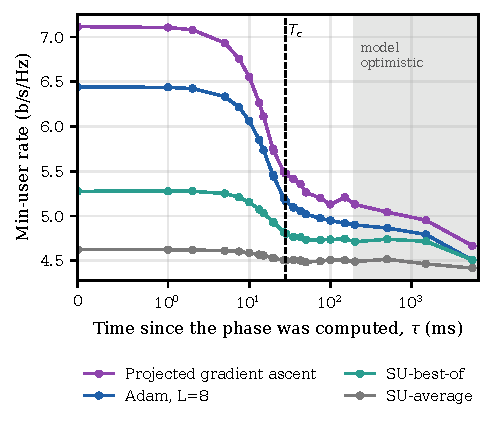
\includegraphics[width=\columnwidth]{figures/fig_aging.pdf}
\caption{Minimum user rate of a phase fixed at $t=0$ as users walk at 1.5~m/s, with the precoder refreshed at every instant. Dashed line: $T_c=28.2$~ms. Shaded: beyond 200~ms the frozen-scatterer model is optimistic.}
\label{fig:aging}
\end{figure}

\subsection{The Intrinsic Optimum}
\label{sec:res_optimum}
Fig.~\ref{fig:optimum} sweeps the number of optimizer steps, starting from SU-average (4.624~b/s/Hz); the point at $L=0$ shows SU-best-of for reference. Adam's $t=0$ rate grows monotonically with $L$, from 5.412 at $L=1$ to 7.037~b/s/Hz at $L=48$. The effective rate does not. It has a flat top between $L=4$ and $L=6$ (5.980, 5.982 and 5.970~b/s/Hz, at 6.7--10.0~ms); none of the three is significantly below the best, and every other step count is. At $L=48$ (79.8~ms) the effective rate is 5.145~b/s/Hz, 14.0\% (95\% CI 12.5--15.5\%) below the optimum, although the $t=0$ rate there is 13.2\% higher.

In terms of~\eqref{eq:marginal}: going from $L=4$ to $L=6$ adds 0.188~b/s/Hz at $t=0$, but the additional 3.3~ms of aging cost 0.198~b/s/Hz. Beyond $L=6$ the effective rate declines; the only exception is a 0.006~b/s/Hz fluctuation between $L=20$ and $L=24$.

The optimum is not specific to Adam or to its step size. Armijo steepest ascent, at 2.36~ms per step, has its best effective rate at $L=6$ (5.820~b/s/Hz, with $L=4$ not significantly lower). It gains less per step than Adam (6.975 against 7.037~b/s/Hz at $L=48$) and costs more per step, so its best effective rate is 0.162~b/s/Hz (95\% CI 0.121--0.203) below Adam's. Repeating the Adam sweep with step sizes 0.25, 0.75 and 1.0 moves the best point to $L=6$, $4$ and $5$, and running to $L=48$ costs 11.5\%, 13.7\% and 11.3\%.

\begin{figure}[t]
\centering
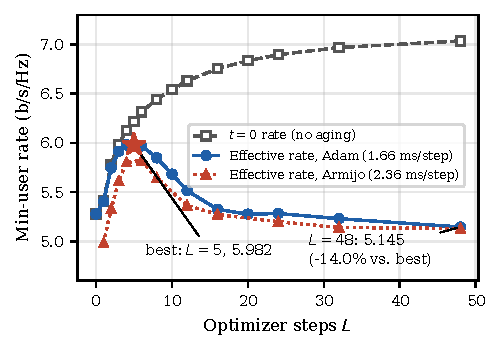
\includegraphics[width=\columnwidth]{figures/fig_intrinsic_optimum.pdf}
\caption{Step sweep on the aging set. Adam's $t=0$ rate increases monotonically, while the effective rate (rate at the method's own completion time) has a flat top at $L=4$--$6$ and is 14.0\% below its best value at $L=48$. Armijo steepest ascent shows the same shape at a lower level. $L=0$: SU-best-of, for reference.}
\label{fig:optimum}
\end{figure}

\subsection{Dependence on the Step Cost}
\label{sec:res_scaling}
The latencies above are those of a single-threaded Python implementation; an optimized implementation would be much faster per step. Fig.~\ref{fig:scaling} therefore scales Adam's per-step latency from 0.01 to 3 times the measured value, which moves the normalized step cost $x=\Delta T f_d$ of~\eqref{eq:x} from $2\times10^{-4}$ to $7\times10^{-2}$; this setup sits at $x=0.025$.

The best step count falls steadily with $x$: 96 steps at $x=2\times10^{-4}$, 48 at $7\times10^{-4}$, 24--32 at $2.5\times10^{-3}$, 12--16 at $7.5\times10^{-3}$, 4--6 here, and 2 at $x=0.075$. Adam's $t=0$ rate saturates near 100 steps (7.087~b/s/Hz at $L=96$, 7.096 at $L=256$), so at the smallest $x$ the optimum is essentially convergence, and running to $L=256$ costs only 1.5\% (95\% CI 1.3--1.8\%). The cost of convergence peaks at about 21\% for $x\approx 2.5\times10^{-3}$, where the optimizer is fast enough to gain much but convergence still takes long. It declines again for large $x$, where even the best policy has little left to gain. For $x\ge 0.025$, $L=256$ lies beyond the 200~ms horizon, so its cost is if anything understated.

The claim that convergence hurts is thus a statement about a regime, not about RIS optimization in general. With a hundredfold faster implementation at pedestrian speed, convergence is nearly free. The same implementation at vehicular speed, or at a millimetre-wave carrier, moves $x$ in the opposite direction.

\begin{figure}[t]
\centering
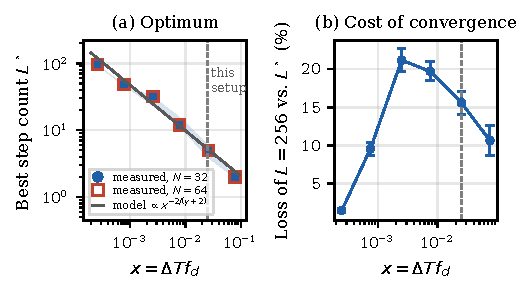
\includegraphics[width=\columnwidth]{figures/fig_step_scaling.pdf}
\caption{Adam on the aging set with its per-step latency scaled from 0.01 to 3 times the measured value. (a)~Best step count; shaded: step counts not significantly below the best. (b)~Effective-rate loss of running to $L=256$ instead of $L^\star$, with 95\% paired bootstrap CIs. Dashed: this setup.}
\label{fig:scaling}
\end{figure}

\subsection{Sensitivity to Acquisition Delay and User Speed}
\label{sec:res_sensitivity}
The effective rate above charges each method only for its own run time. A deployed system also spends time on pilots, estimation and feedback before the optimizer starts, which for this system is between about 1 and 10~ms (Section~\ref{sec:method}). We therefore add an acquisition delay $T_{\mathrm{ov}}$ to every latency and repeat the sweep at four user speeds (Table~\ref{tab:sens}). The direction is the one predicted by~\eqref{eq:marginal}: a faster channel or a longer delay makes each additional step cost more aging, and the optimum moves to fewer steps. Without delay, the near-optimal range shifts from $L=6$--$8$ at 1~m/s to $L=3$ at 3~m/s, and at 1.5~m/s it shifts from $L=4$--$6$ to $L=3$--$4$ as $T_{\mathrm{ov}}$ grows from 0 to 10~ms. The best effective rate falls with $T_{\mathrm{ov}}$ at every speed. We do not interpret cells with $T_{\mathrm{ov}} > T_c/2$, where the channel has largely changed before optimization starts. The only such cell is 3~m/s with 10~ms; there all step counts give rates within 0.26~b/s/Hz, and the maximum falls at $L=32$, which carries no meaning. In all other cells, running Adam to $L=48$ costs 2.9--14.7\% of the attainable effective rate.

The optimum is also tolerant of an error in the assumed speed. Choosing $L$ for 1.5~m/s when users actually move at 1.8~m/s, or the reverse, costs less than 0.5\% of the attainable effective rate. The largest loss in our grid, 5.7\%, occurs when $L$ is chosen for 1~m/s and users move at 3~m/s.

\begin{table}[t]
\centering
\caption{Best number of Adam steps $L^\star$ on the grid $L\in\{1,\dots,6,8,10,12,16,20,24,32,48\}$ and, in parentheses, the range of $L$ within 0.5\% of the best effective rate, for different user speeds and channel-acquisition delays $T_{\mathrm{ov}}$ (aging set). $^\ddagger$$T_{\mathrm{ov}} > T_c/2$: not interpreted.}
\label{tab:sens}
\footnotesize
\setlength{\tabcolsep}{4pt}
\begin{tabular}{lrrrrr}
\toprule
& \multicolumn{5}{c}{Acquisition delay $T_{\mathrm{ov}}$ (ms)} \\
$v$ (m/s), $T_c$ & 0 & 1 & 2 & 5 & 10 \\
\midrule
1, 42.3~ms & 6 (6--8) & 6 (6--8) & 6 (5--8) & 6 (5--6) & 5 (4--6) \\
1.5, 28.2~ms & 5 (4--6) & 4 (4--5) & 4 (4--5) & 4 (3--4) & 3 (3--4) \\
1.8, 23.5~ms & 4 (4--5) & 4 (3--4) & 4 (3--4) & 3 (3--4) & 3 (3--4) \\
3, 14.1~ms & 3 (3) & 3 (3) & 3 (2--3) & 2 (2--3) & 32$^\ddagger$ (32--48) \\
\bottomrule
\end{tabular}

\end{table}

\subsection{Periodic Re-optimization}
\label{sec:res_tracking}
Table~\ref{tab:tracking} simulates a controller that re-optimizes continuously (Definition~3) on a 0.5~ms grid over 200~ms, averaging the minimum user rate over 50--200~ms so that the start-up cycles do not dominate. Each phase is now used for a whole cycle, which penalizes long cycles twice: the phase is older when it arrives and it stays in use longer. Accordingly, the best cold-start policy uses $L=3$ steps per cycle, fewer than the single-shot optimum. Warm starts accumulate progress across cycles, so even shorter cycles pay off. Two warm-started steps per cycle give 6.350~b/s/Hz at $T_{\mathrm{ov}}=0$, 0.52~b/s/Hz more than the best cold-start policy. The same ordering holds with 2 and 5~ms of acquisition delay. With 48 steps per cycle, warm starting no longer helps (5.02~b/s/Hz in both cases), and the time-averaged rate is 13.8\% (cold) and 20.9\% (warm) below the best policy.

\begin{table}[t]
\centering
\caption{Time-averaged effective rate (Definition~3, b/s/Hz, 50--200~ms) of a controller that re-optimizes continuously with $L$ Adam steps per cycle, cold- or warm-started, for three acquisition delays (aging set). Bold: not significantly below the best $L$ of the column (paired bootstrap, 95\%).}
\label{tab:tracking}
\footnotesize
\setlength{\tabcolsep}{4pt}
\begin{tabular}{rrrrrrr}
\toprule
 & \multicolumn{2}{c}{$T_{\mathrm{ov}}=0$~ms} & \multicolumn{2}{c}{$T_{\mathrm{ov}}=2$~ms} & \multicolumn{2}{c}{$T_{\mathrm{ov}}=5$~ms} \\
$L$ & cold & warm & cold & warm & cold & warm \\
\midrule
1 & 5.40 & 6.06 & 5.36 & 5.88 & 5.25 & 5.62 \\
2 & 5.73 & \textbf{6.35} & 5.64 & \textbf{6.15} & 5.46 & \textbf{5.84} \\
3 & \textbf{5.83} & 6.31 & \textbf{5.70} & 6.10 & \textbf{5.48} & 5.79 \\
4 & \textbf{5.82} & 6.18 & 5.66 & 5.97 & 5.44 & 5.68 \\
6 & 5.69 & 5.92 & 5.53 & 5.74 & 5.34 & 5.52 \\
8 & 5.49 & 5.66 & 5.37 & 5.53 & 5.25 & 5.38 \\
12 & 5.28 & 5.38 & 5.26 & 5.32 & 5.20 & 5.26 \\
16 & 5.23 & 5.28 & 5.20 & 5.25 & 5.17 & 5.22 \\
24 & 5.18 & 5.20 & 5.16 & 5.20 & 5.16 & 5.17 \\
48 & 5.03 & 5.02 & 5.01 & 5.01 & 4.99 & 4.99 \\
\bottomrule
\end{tabular}

\end{table}

\subsection{Learned versus Classical: Equal Steps and Equal Milliseconds}
\label{sec:res_reversal}
This comparison is made on the static set, without mobility, and with $t=0$ rates. It isolates the question of compute efficiency, which the previous subsections show to be what matters once latency enters. The learned model was not evaluated on the aging set.

Table~\ref{tab:eqstep} compares the learned update rule with tuned Adam at equal step counts on the static test set; both start from SU-average (3.539~b/s/Hz). The learned rule is ahead at every budget, the paired difference minus two standard errors is positive at every budget, and it wins on 68--84\% of test scenarios. On a step axis, the learned rule is the better optimizer.

\begin{table}[t]
\centering
\caption{Equal number of steps, static test set (600 scenarios). Adam step size and objective selected on 400 validation scenarios at each $L$.}
\label{tab:eqstep}
\footnotesize
\begin{tabular}{rrrrrr}
\toprule
$L$ & Learned & Adam & Ratio & Diff.\,$-2$\,s.e. & Wins \\
 & (b/s/Hz) & (b/s/Hz) & & (b/s/Hz) & (\%) \\
\midrule
1 & 4.460 & 4.381 & 1.018 & +0.061 & 74.8 \\
2 & 4.879 & 4.693 & 1.040 & +0.160 & 83.2 \\
4 & 5.285 & 5.025 & 1.052 & +0.228 & 83.7 \\
8 & 5.593 & 5.380 & 1.040 & +0.184 & 83.2 \\
16 & 5.800 & 5.739 & 1.011 & +0.039 & 68.3 \\
\bottomrule
\end{tabular}

\end{table}

Steps, however, are not equally expensive. One learned step takes 4.6--6.5~ms, one Adam step 1.60--1.71~ms, so a learned step costs 2.7--4.0 Adam steps. Table~\ref{tab:eqms} and Fig.~\ref{fig:eqms}(b) place both methods on the measured latency axis. Every learned configuration is dominated by an Adam configuration that is both faster and better. This holds in each of the five timing rounds separately, although not always by the configuration listed: for learned $L=16$, Adam with $L=48$ is slower in two rounds, and Adam with $L=32$ (6.013~b/s/Hz, at most 62.97~ms) dominates in every round. For example, the learned rule with $L=4$ needs 18.41~ms for 5.285~b/s/Hz, while Adam with $L=8$ needs 13.48~ms for 5.380~b/s/Hz. The ranking from the equal-step comparison reverses completely.

Three remarks bound this result. First, aging was not included; since the learned configuration is the slower one in every pair, aging would be expected to widen rather than close the gap, but we have not measured this. Second, the learned timing excludes feature computation, so the latency gap is if anything understated. Third, the cost ratio is a property of this implementation: on hardware that accelerates the network's matrix products more than Adam's step, the reversal could weaken.

\begin{table}[t]
\centering
\caption{Equal milliseconds: each learned configuration and the best Adam configuration that dominates it (lower median latency and higher rate). Medians over five rounds. In every round each learned configuration is dominated by at least one Adam configuration.}
\label{tab:eqms}
\footnotesize
\begin{tabular}{rrr|rrr}
\toprule
\multicolumn{3}{c|}{Learned update} & \multicolumn{3}{c}{Dominating Adam} \\
$L$ & ms & b/s/Hz & $L$ & ms & b/s/Hz \\
\midrule
1 & 5.16 & 4.460 & 2 & 3.20 & 4.693 \\
2 & 12.95 & 4.879 & 4 & 6.49 & 5.025 \\
4 & 18.41 & 5.285 & 8 & 13.48 & 5.380 \\
8 & 36.76 & 5.593 & 16 & 27.31 & 5.739 \\
16 & 83.80 & 5.800 & 48 & 78.77 & 6.107 \\
\bottomrule
\end{tabular}

\end{table}

\begin{figure*}[t]
\centering
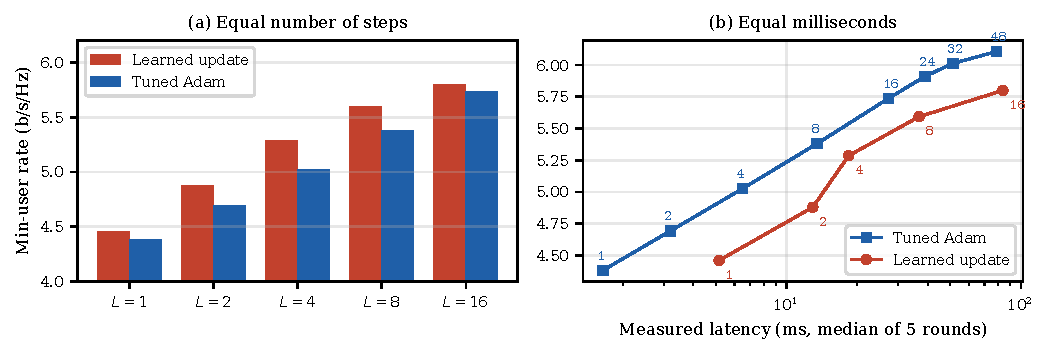
\includegraphics[width=\textwidth]{figures/fig_equal_step_vs_ms.pdf}
\caption{Learned update rule versus tuned Adam on the static test set. (a)~At an equal number of steps, the learned rule is ahead at every budget. (b)~On the measured latency axis (numbers: steps), every learned configuration lies below and to the right of the Adam curve, i.e., it is dominated.}
\label{fig:eqms}
\end{figure*}

\subsection{What the Fresh-Beam Assumption Is Worth}
\label{sec:res_beam}
All results above assume that the BS precoder is recomputed from the current channel while only the RIS phase ages (Section~\ref{sec:framework}). Table~\ref{tab:beam} and Fig.~\ref{fig:beam} measure the alternative in which the precoder ages too, on the separate beam set (Section~\ref{sec:method}), whose absolute rates are not comparable with Table~\ref{tab:aging}. Both curves use the same $t=0$ phase. With a fresh beam the rate decays moderately (Adam with $L=8$: from 5.342 to 4.358~b/s/Hz at $T_c$); with a stale beam it collapses within tens of milliseconds, and at $T_c$ it is 11.7--14.2$\times$ lower than with a fresh beam, for every phase choice. The assumption therefore matters, and it must hold in a deployment for the effective rates above to apply: the BS has to refresh its precoder at least once per coherence time. Refreshing it is cheap: single-threaded, computing the effective channel and the regularized ZF precoder takes a median of 0.12~ms, about 13$\times$ less than a single Adam step (8.0--15.0$\times$ across five rounds). We have not included this time in the effective rates. This is the usual frame-by-frame operation of a multi-antenna BS, but it is an assumption of our results rather than a finding.

\begin{table}[t]
\centering
\caption{Fresh versus stale precoder at $\tau=T_c=28.2$~ms, phase fixed at $t=0$ in both (beam set, 400 scenarios).}
\label{tab:beam}
\footnotesize
\begin{tabular}{lrrr}
\toprule
Phase chosen at $t=0$ & Fresh beam & Stale beam & Ratio \\
 & (b/s/Hz) & (b/s/Hz) & \\
\midrule
SU-average & 3.586 & 0.306 & 11.7$\times$ \\
SU-best-of & 3.924 & 0.305 & 12.9$\times$ \\
Adam, $L=8$ & 4.358 & 0.307 & 14.2$\times$ \\
\bottomrule
\end{tabular}

\end{table}

\begin{figure}[t]
\centering
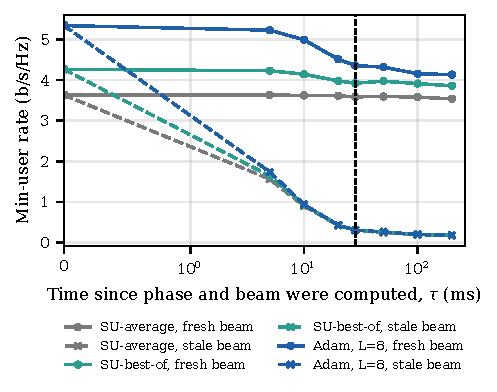
\includegraphics[width=\columnwidth]{figures/fig_beam_staleness.pdf}
\caption{Same $t=0$ phase evaluated with a precoder recomputed from the current channel (fresh) or kept from $t=0$ (stale). Dashed line: $T_c$.}
\label{fig:beam}
\end{figure}
